\documentclass[tikz,border=10pt]{standalone}
% Shared preamble for the bootqcc TikZ figures.
\usepackage[T1]{fontenc}
\usepackage{helvet}
\renewcommand{\familydefault}{\sfdefault}
\usepackage{amsmath}
\usetikzlibrary{arrows.meta,positioning,shapes.geometric,fit,backgrounds,calc}

\definecolor{navy}{HTML}{1F3A5F}
\definecolor{sky}{HTML}{5AA9E6}
\definecolor{coral}{HTML}{FF6B6B}
\definecolor{slate}{HTML}{6B7A8F}

\tikzset{
  box/.style={rectangle, rounded corners=4pt, draw=navy, fill=sky!15, thick,
              align=center, minimum height=1.0cm, inner sep=6pt, text width=4.6cm},
  inbox/.style={rectangle, rounded corners=4pt, draw=slate, fill=slate!10, thick,
              align=center, minimum height=0.9cm, inner sep=5pt, text width=3.0cm,
              font=\small},
  io/.style={trapezium, trapezium left angle=72, trapezium right angle=108,
             draw=navy, fill=white, thick, align=center, minimum height=1.2cm,
             inner sep=5pt, text width=3.0cm},
  result/.style={rectangle, rounded corners=8pt, draw=coral, fill=coral!10, thick,
              align=center, minimum height=1.0cm, inner sep=6pt, text width=4.0cm},
  term/.style={rectangle, rounded corners=12pt, draw=navy, fill=navy, text=white,
               thick, align=center, minimum height=0.9cm, inner sep=6pt, text width=4.2cm},
  dec/.style={diamond, aspect=2.6, draw=navy, fill=white, thick, align=center,
              inner sep=0pt, text width=2.7cm, font=\small},
  err/.style={rectangle, rounded corners=4pt, draw=coral, fill=coral!15, thick,
              align=center, minimum height=0.9cm, inner sep=6pt, text width=3.2cm},
  arr/.style={-{Latex[length=3mm]}, thick, navy},
  lab/.style={font=\footnotesize\bfseries, text=navy, fill=white, inner sep=1.5pt},
  phase/.style={rounded corners=8pt, draw=navy!45, dashed, thick, inner sep=12pt},
}

\tikzset{
  mbox/.style={box, text width=5.5cm, font=\small, inner sep=5pt},
  stage/.style={rounded corners=10pt, draw=navy!45, fill=navy!3, thick, inner sep=12pt},
  smallbox/.style={box, text width=2.2cm, font=\small, inner sep=4pt},
}
\newcommand{\refs}[1]{\\[2pt]{\scriptsize\itshape\color{slate}#1}}
\newcommand{\badge}[1]{\tikz[baseline=(c.base)]\node[circle,fill=navy,text=white,inner sep=2pt,font=\bfseries\small](c){#1};}

\begin{document}
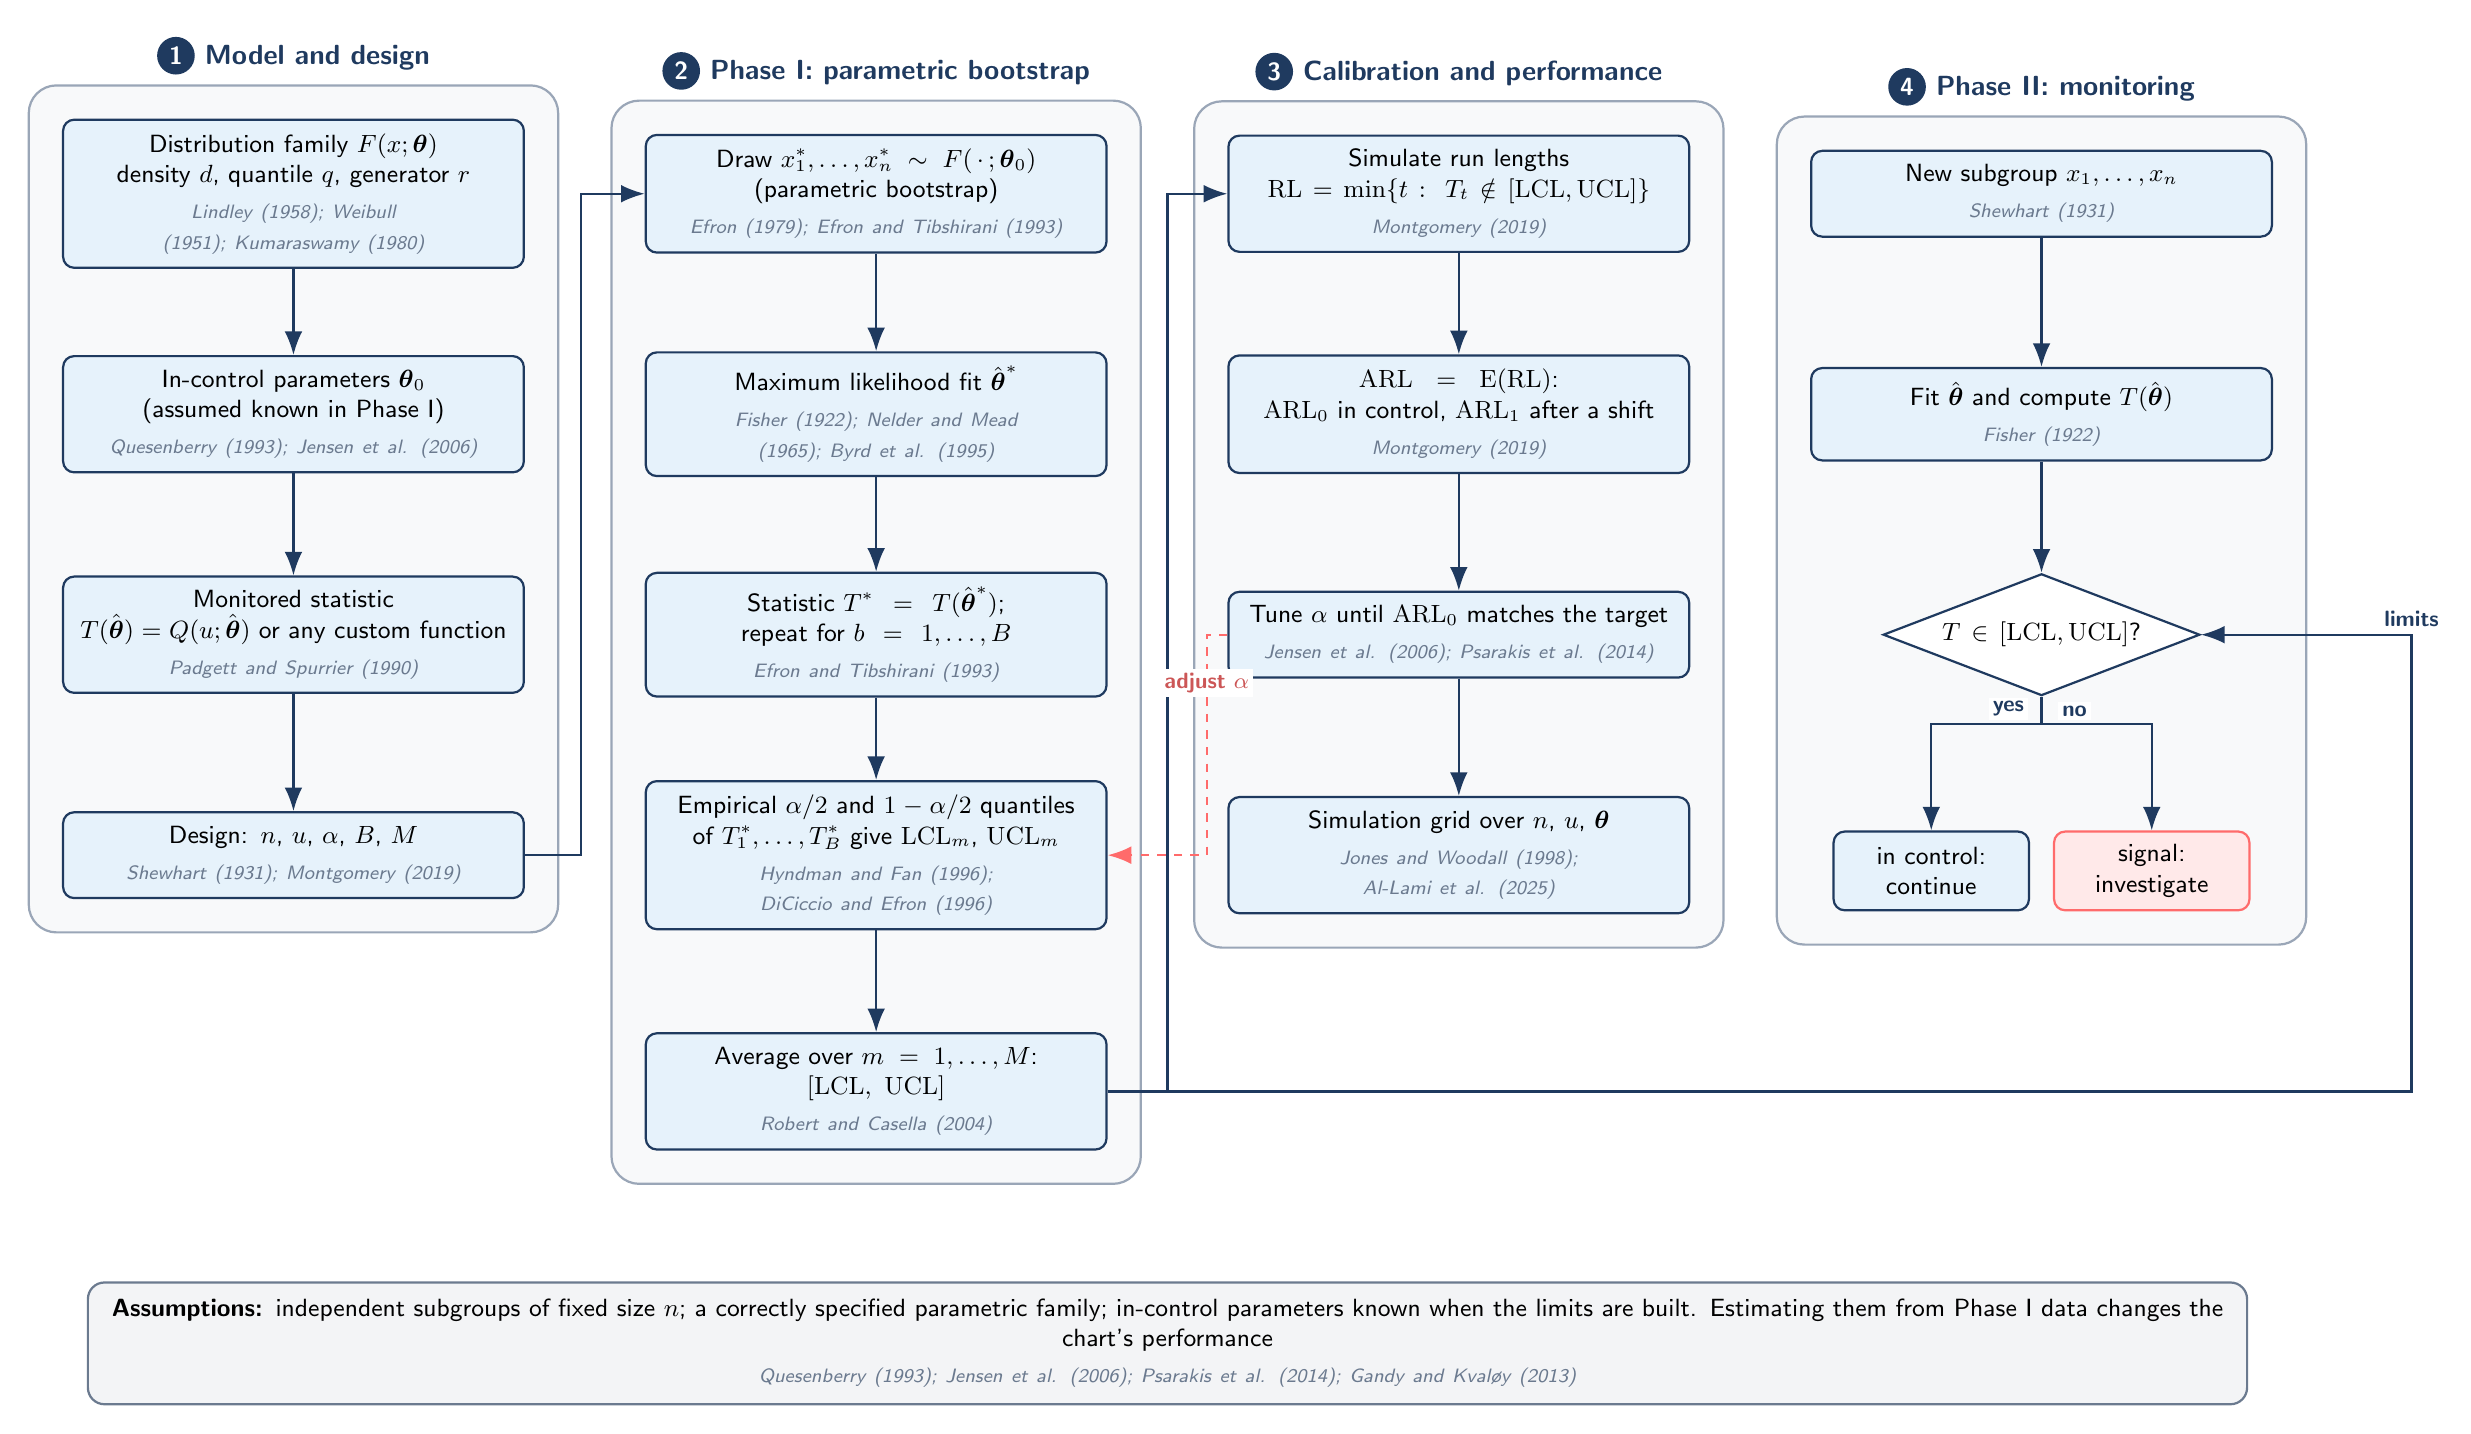
\begin{tikzpicture}

  % ------------------------------------------------------------ stage 1
  \node[mbox] (a1) at (0,0)
    {Distribution family $F(x;\boldsymbol\theta)$\\ density $d$, quantile $q$, generator $r$%
     \refs{Lindley (1958); Weibull (1951); Kumaraswamy (1980)}};
  \node[mbox] (a2) at (0,-2.8)
    {In-control parameters $\boldsymbol\theta_0$\\ (assumed known in Phase I)%
     \refs{Quesenberry (1993); Jensen et al. (2006)}};
  \node[mbox] (a3) at (0,-5.6)
    {Monitored statistic\\ $T(\hat{\boldsymbol\theta})=Q(u;\hat{\boldsymbol\theta})$ or any custom function%
     \refs{Padgett and Spurrier (1990)}};
  \node[mbox] (a4) at (0,-8.4)
    {Design: $n$, $u$, $\alpha$, $B$, $M$%
     \refs{Shewhart (1931); Montgomery (2019)}};

  % ------------------------------------------------------------ stage 2
  \node[mbox] (b1) at (7.4,0)
    {Draw $x^*_1,\dots,x^*_n\sim F(\,\cdot\,;\boldsymbol\theta_0)$ (parametric bootstrap)%
     \refs{Efron (1979); Efron and Tibshirani (1993)}};
  \node[mbox] (b2) at (7.4,-2.8)
    {Maximum likelihood fit $\hat{\boldsymbol\theta}^*$%
     \refs{Fisher (1922); Nelder and Mead (1965); Byrd et al. (1995)}};
  \node[mbox] (b3) at (7.4,-5.6)
    {Statistic $T^*=T(\hat{\boldsymbol\theta}^*)$;\\ repeat for $b=1,\dots,B$%
     \refs{Efron and Tibshirani (1993)}};
  \node[mbox] (b4) at (7.4,-8.4)
    {Empirical $\alpha/2$ and $1-\alpha/2$ quantiles of $T^*_1,\dots,T^*_B$ give $\mathrm{LCL}_m$, $\mathrm{UCL}_m$%
     \refs{Hyndman and Fan (1996); DiCiccio and Efron (1996)}};
  \node[mbox] (b5) at (7.4,-11.4)
    {Average over $m=1,\dots,M$:\\ $[\mathrm{LCL},\ \mathrm{UCL}]$%
     \refs{Robert and Casella (2004)}};

  % ------------------------------------------------------------ stage 3
  \node[mbox] (c1) at (14.8,0)
    {Simulate run lengths\\ $\mathrm{RL}=\min\{t:\ T_t\notin[\mathrm{LCL},\mathrm{UCL}]\}$%
     \refs{Montgomery (2019)}};
  \node[mbox] (c2) at (14.8,-2.8)
    {$\mathrm{ARL}=\operatorname{E}(\mathrm{RL})$:\\ $\mathrm{ARL}_0$ in control, $\mathrm{ARL}_1$ after a shift%
     \refs{Montgomery (2019)}};
  \node[mbox] (c3) at (14.8,-5.6)
    {Tune $\alpha$ until $\mathrm{ARL}_0$ matches the target%
     \refs{Jensen et al. (2006); Psarakis et al. (2014)}};
  \node[mbox] (c4) at (14.8,-8.4)
    {Simulation grid over $n$, $u$, $\boldsymbol\theta$%
     \refs{Jones and Woodall (1998); Al-Lami et al. (2025)}};

  % ------------------------------------------------------------ stage 4
  \node[mbox] (d1) at (22.2,0)
    {New subgroup $x_1,\dots,x_n$%
     \refs{Shewhart (1931)}};
  \node[mbox] (d2) at (22.2,-2.8)
    {Fit $\hat{\boldsymbol\theta}$ and compute $T(\hat{\boldsymbol\theta})$%
     \refs{Fisher (1922)}};
  \node[dec, text width=3.2cm] (d3) at (22.2,-5.6) {$T\in[\mathrm{LCL},\mathrm{UCL}]$?};
  \node[smallbox, fill=sky!15] (d4) at (20.8,-8.6) {in control:\\ continue};
  \node[smallbox, draw=coral, fill=coral!15] (d5) at (23.6,-8.6) {signal:\\ investigate};

  % ------------------------------------------------------------ stage frames
  \begin{pgfonlayer}{background}
    \node[stage, fit=(a1)(a4), label={[navy,font=\bfseries]above:\badge{1}\ Model and design}] (s1) {};
    \node[stage, fit=(b1)(b5), label={[navy,font=\bfseries]above:\badge{2}\ Phase I: parametric bootstrap}] (s2) {};
    \node[stage, fit=(c1)(c4), label={[navy,font=\bfseries]above:\badge{3}\ Calibration and performance}] (s3) {};
    \node[stage, fit=(d1)(d4)(d5), label={[navy,font=\bfseries]above:\badge{4}\ Phase II: monitoring}] (s4) {};
  \end{pgfonlayer}

  % ------------------------------------------------------------ arrows inside stages
  \foreach \u/\v in {a1/a2,a2/a3,a3/a4,b1/b2,b2/b3,b3/b4,b4/b5,c1/c2,c2/c3,c3/c4,d1/d2,d2/d3}
    \draw[arr] (\u) -- (\v);
  \draw[arr] (d3.south) -- ++(0,-0.35) -| node[lab, pos=0.15, above=1pt] {yes} (d4.north);
  \draw[arr] (d3.south) -- ++(0,-0.35) -| node[lab, pos=0.15, above=1pt] {no} (d5.north);

  % ------------------------------------------------------------ arrows between stages
  \draw[arr] (a4.east) -- (3.65,-8.4) |- (b1.west);
  \draw[arr] (b5.east) -- (11.1,-11.4) |- (c1.west);
  \draw[arr, coral, dashed] (c3.west) -- (11.6,-5.6) |- node[lab, pos=0.15, above=1pt, text=coral!80!black] {adjust $\alpha$} (b4.east);
  \draw[arr] (b5.east) -- (26.9,-11.4) |- node[lab, pos=0.5, above=1pt] {limits} (d3.east);

  % ------------------------------------------------------------ assumptions band
  \node[rectangle, rounded corners=6pt, draw=slate, fill=slate!8, thick, align=center,
        text width=27cm, inner sep=6pt, font=\small] at (11.1,-14.6)
    {\textbf{Assumptions:} independent subgroups of fixed size $n$; a correctly specified parametric
     family; in-control parameters known when the limits are built. Estimating them from Phase I data
     changes the chart's performance%
     \refs{Quesenberry (1993); Jensen et al. (2006); Psarakis et al. (2014); Gandy and Kval{\o}y (2013)}};
\end{tikzpicture}
\end{document}
